\section{Respuesta a las preguntas de negocio}
Las ocho preguntas de negocio planteadas en la Entrega 1 se responden en esta sección utilizando la vista minable Gold como insumo único. El procesamiento estadístico (agregaciones, correlaciones de Pearson, particiones por cuartil) se realiza directamente en Spark mediante el DataFrame API, y los visuales de respaldo se generan a partir de los resultados ya computados. La trazabilidad completa de cada pregunta está disponible en el notebook \texttt{07\_eda\_y\_preguntas\_negocio} del repositorio.

\subsection{Q1. Relación entre el acceso a internet en el hogar y el desempeño Saber 11 a nivel municipal}
La correlación de Pearson entre el porcentaje de estudiantes con internet en casa (\texttt{pct\_internet\_icfes}) y el puntaje global promedio del municipio (\texttt{avg\_punt\_global}) es de $r = +0.4092$, calculada sobre las 7,001 observaciones municipio-año válidas. Se trata de una correlación moderada y positiva, lo que confirma cuantitativamente la hipótesis central del proyecto: a mayor penetración de internet en los hogares, mayor el puntaje promedio del municipio.

\begin{table}[H]
\centering
\caption{Puntaje global promedio por cuartil de penetración de internet en el hogar.}
\begin{tabular}{l r r}
\toprule
\textbf{Cuartil de internet} & \textbf{Puntaje promedio} & \textbf{N° municipios-año} \\
\midrule
Q1 (bajo)  & 233.02 & 1,727 \\
Q2         & 236.86 & 1,718 \\
Q3         & 239.00 & 1,751 \\
Q4 (alto)  & 252.09 & 1,808 \\
\bottomrule
\end{tabular}
\end{table}

La progresión es monótona y muestra una diferencia neta de cerca de 19 puntos entre el cuartil más bajo y el más alto. El salto más pronunciado ocurre entre el tercer y el cuarto cuartil, lo que sugiere que el beneficio del acceso al internet doméstico no es lineal sino que se concentra en los municipios donde la penetración supera un umbral cercano al 42\%.

\begin{figure}[H]
\centering
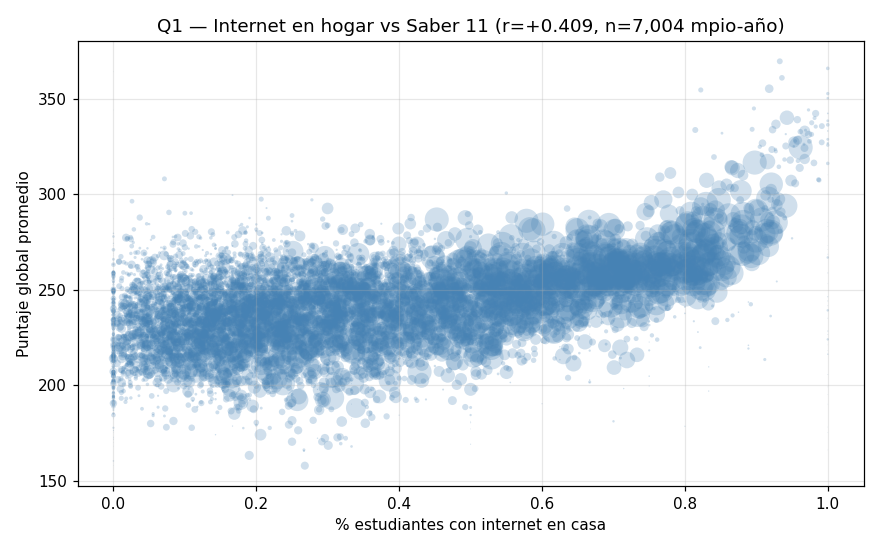
\includegraphics[width=0.85\textwidth]{figures/q1_internet_vs_puntaje.png}
\caption{Q1. Dispersión municipio-año entre porcentaje de estudiantes con internet en casa y puntaje global promedio. El tamaño del punto representa el número de estudiantes evaluados.}
\end{figure}

\subsection{Q2. Variación del rendimiento entre zonas rurales y urbanas en función de la conectividad}
Para responder esta pregunta se construyó una tabla cruzada entre la categoría de zona del municipio (rural si el porcentaje de colegios rurales es mayor o igual a 50\%, urbano/mixto en otro caso) y el cuartil de penetración de internet. El resultado evidencia que la brecha rural-urbana persiste, pero el patrón no es uniforme.

\begin{table}[H]
\centering
\caption{Puntaje global promedio por zona y cuartil de internet.}
\begin{tabular}{l r r r r}
\toprule
\textbf{Zona} & \textbf{Q1 (bajo)} & \textbf{Q2} & \textbf{Q3} & \textbf{Q4 (alto)} \\
\midrule
Rural        & 227.82 & 231.70 & 229.26 & 257.59 \\
Urbano/Mixto & 235.27 & 238.48 & 241.19 & 251.21 \\
\bottomrule
\end{tabular}
\end{table}

Lo más relevante de este resultado es que en el cuartil superior de conectividad la zona rural alcanza un puntaje promedio (257.59) que iguala e incluso supera ligeramente al promedio urbano (251.21) del mismo cuartil. Esto sugiere que cuando la conectividad rural llega a niveles altos, su efecto compensador es notable y puede cerrar la brecha territorial. La conclusión de negocio es clara: invertir en conectividad de alto nivel en zonas rurales es una palanca con retorno comprobable en términos académicos.

\begin{figure}[H]
\centering
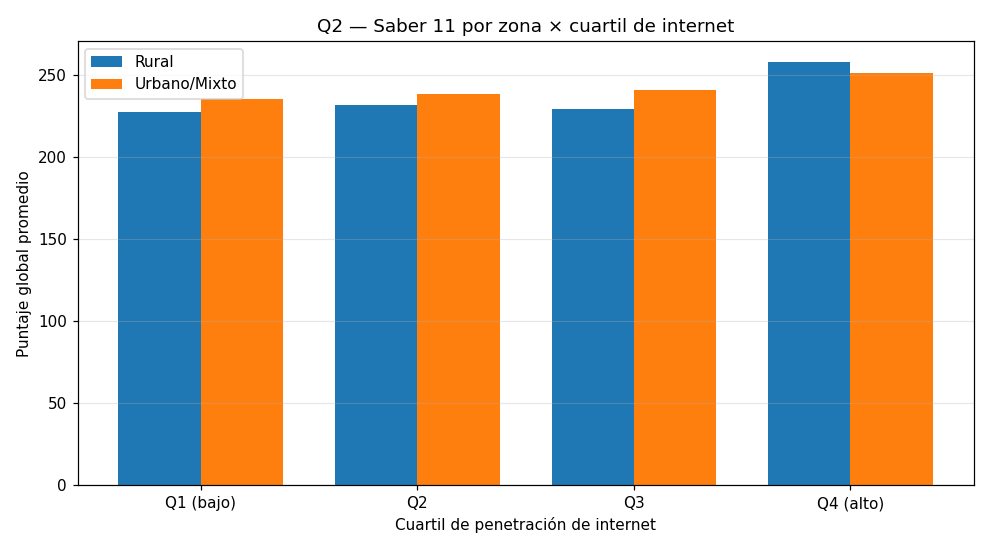
\includegraphics[width=0.85\textwidth]{figures/q2_zona_x_internet.png}
\caption{Q2. Puntaje global promedio por zona y cuartil de penetración de internet.}
\end{figure}

\subsection{Q3. Pobreza multidimensional y resultados académicos, controlando por internet}
Esta pregunta busca determinar si el efecto de la pobreza multidimensional sobre el rendimiento académico se mantiene aun cuando se controla por el nivel de conectividad. Para responderla, se estratificó la base por cuartil de internet y, dentro de cada estrato, se calculó la correlación entre el índice de privación Sisbén y el puntaje global promedio.

\begin{table}[H]
\centering
\caption{Correlación entre índice de privación Sisbén y puntaje global, dentro de cada cuartil de internet.}
\begin{tabular}{l r r r}
\toprule
\textbf{Cuartil de internet} & \textbf{N° municipios-año} & \textbf{Corr (privación, puntaje)} & \textbf{Puntaje promedio} \\
\midrule
Q1 (bajo)  & 1,661 & $-0.461$ & 234.1 \\
Q2         & 1,702 & $-0.510$ & 237.2 \\
Q3         & 1,745 & $-0.521$ & 239.2 \\
Q4 (alto)  & 1,805 & $-0.404$ & 252.2 \\
\midrule
Sin controlar por internet & 6,913 & $-0.520$ & --- \\
\bottomrule
\end{tabular}
\end{table}

El resultado es contundente: la correlación entre privación y puntaje se mantiene negativa y estadísticamente significativa en los cuatro estratos, con magnitudes que oscilan entre $-0.40$ y $-0.52$. Esto confirma que la pobreza multidimensional incide en el desempeño académico \textbf{independientemente del nivel de conectividad} del municipio: incluso en los territorios mejor conectados, los municipios con mayor privación obtienen sistemáticamente puntajes más bajos. La conectividad no es un sustituto del bienestar socioeconómico, sino un complemento.

\subsection{Q4. Diferencias entre municipios con alta y baja penetración de internet}
Para cuantificar la diferencia entre los extremos de conectividad, se definieron dos grupos: el grupo de \textbf{alta} penetración corresponde al 20\% superior de \texttt{pct\_internet\_icfes} (percentil 80 o superior) y el grupo de \textbf{baja} corresponde al 20\% inferior (percentil 20 o inferior).

\begin{table}[H]
\centering
\caption{Comparativa de los grupos de alta y baja penetración de internet.}
\begin{tabular}{l r r}
\toprule
\textbf{Indicador} & \textbf{Grupo ALTA} & \textbf{Grupo BAJA} \\
\midrule
Puntaje global promedio              & 250.4 & 228.3 \\
Penetración de internet (promedio)   & 0.681 & 0.099 \\
Índice de privación promedio         & 3.06  & 4.92  \\
\bottomrule
\end{tabular}
\end{table}

La diferencia neta de puntaje entre los dos grupos es de $+22.1$ puntos a favor del grupo de alta conectividad. Adicionalmente, el grupo de alta penetración presenta un índice de privación significativamente menor, lo que refuerza el hallazgo de Q3: alta conectividad y baja privación coexisten en los municipios más exitosos académicamente.

\subsection{Q5. Variables socioeconómicas con mayor capacidad explicativa frente al acceso a internet}
Se calculó la correlación de Pearson entre cada feature candidata y el puntaje global, y se ranquearon por valor absoluto. El resultado muestra que el acceso a internet, aunque relevante, no es la variable con mayor poder explicativo.

\begin{table}[H]
\centering
\caption{Ranking de correlación de Pearson con el puntaje global promedio del municipio.}
\begin{tabular}{l r}
\toprule
\textbf{Variable}                  & \textbf{Correlación} \\
\midrule
pct\_grupo\_D (Sisbén)             & $+0.4235$ \\
\textbf{pct\_internet\_icfes}      & $\mathbf{+0.4092}$ \\
idx\_privacion (Sisbén)            & $-0.3775$ \\
pct\_grupo\_A (Sisbén)             & $-0.3429$ \\
pct\_rural\_colegio                & $-0.1752$ \\
COBERTURA\_NETA                    & $+0.1636$ \\
pct\_rural\_sisben                 & $+0.1560$ \\
accesos\_per\_capita\_5\_16        & $+0.1398$ \\
DESERCION                          & $-0.1287$ \\
POBLACION\_5\_16                   & $+0.1074$ \\
n\_estudiantes                     & $+0.0835$ \\
avg\_velocidad\_bajada             & $+0.0707$ \\
APROBACION                         & $+0.0639$ \\
\bottomrule
\end{tabular}
\end{table}

La variable con mayor correlación positiva es el porcentaje de personas clasificadas en el grupo D del Sisbén (el menos vulnerable), con $r = +0.4235$, ligeramente superior al porcentaje de estudiantes con internet en casa ($r = +0.4092$). Esto indica que el peso socioeconómico estructural medido por el Sisbén compite con la conectividad como variable explicativa. En sentido inverso, el índice de privación ($r = -0.3775$) y el porcentaje en grupo A ($r = -0.3429$) son las variables que más penalizan el desempeño. La conclusión es que la política pública no puede limitarse a invertir en conectividad: debe contemplar simultáneamente intervenciones sobre las condiciones de vulnerabilidad socioeconómica.

\subsection{Q6. Relación entre la cobertura educativa y la conectividad}
La correlación entre la cobertura neta MEN y la penetración de internet en el hogar es de $r = +0.2415$, mientras que la correlación entre la tasa de matriculación 5-16 años y la conectividad es de $r = +0.2556$. Ambas son correlaciones positivas y moderadas, lo que sugiere que los municipios con mayor cobertura educativa tienden a tener también mayor penetración de internet, posiblemente porque comparten factores estructurales comunes (urbanización, capacidad fiscal, presencia institucional).

\begin{table}[H]
\centering
\caption{Conectividad y puntaje promedio por cuartil de cobertura neta del MEN.}
\begin{tabular}{l r r r}
\toprule
\textbf{Cuartil de cobertura} & \textbf{N° mpio-año} & \textbf{Penetración promedio} & \textbf{Puntaje promedio} \\
\midrule
Q1 (bajo)  & 1,728 & 0.275 & 236.97 \\
Q2         & 1,727 & 0.331 & 240.62 \\
Q3         & 1,726 & 0.355 & 243.45 \\
Q4 (alto)  & 1,727 & 0.376 & 240.86 \\
\bottomrule
\end{tabular}
\end{table}

El patrón es ascendente entre los tres primeros cuartiles pero se aplana en el cuarto, lo que sugiere rendimientos decrecientes: una vez que la cobertura educativa supera cierto umbral, la conectividad adicional ya no se traduce automáticamente en mejoras de puntaje.

\subsection{Q7. Influencia del acceso a computador en el hogar sobre los resultados por área evaluada}
Esta pregunta opera a nivel estudiante individual (no municipal), por lo que se procesa sobre los 4,500,067 registros del Silver ICFES. Los estudiantes se separan en dos grupos según la variable binaria \texttt{TIENE\_COMPUTADOR\_BIN}: 2,569,388 (57.1\%) tienen computador en casa y 1,930,679 (42.9\%) no. El puntaje promedio se calcula por área evaluada para cada grupo.

\begin{table}[H]
\centering
\caption{Puntaje promedio por área evaluada según acceso a computador en el hogar.}
\begin{tabular}{l r r r}
\toprule
\textbf{Área evaluada}        & \textbf{Sin computador} & \textbf{Con computador} & \textbf{Diferencia} \\
\midrule
Lectura crítica               & 48.93 & 54.63 & $+5.70$ \\
Matemáticas                   & 47.00 & 53.55 & $+6.55$ \\
Ciencias naturales            & 46.76 & 52.62 & $+5.86$ \\
Sociales y ciudadanas         & 45.19 & 51.63 & $+6.44$ \\
Inglés                        & 45.61 & 53.86 & $+8.25$ \\
\bottomrule
\end{tabular}
\end{table}

El efecto del computador en casa es positivo en \textbf{todas las áreas evaluadas}, sin excepción. La mayor brecha se observa en inglés ($+8.25$ puntos), seguida por matemáticas ($+6.55$) y sociales ($+6.44$). Estos resultados sugieren que el computador no solo facilita el acceso a contenidos académicos generales, sino que tiene un efecto diferencial en áreas que requieren práctica autónoma e interacción con recursos digitales especializados, como el aprendizaje del inglés.

\begin{figure}[H]
\centering
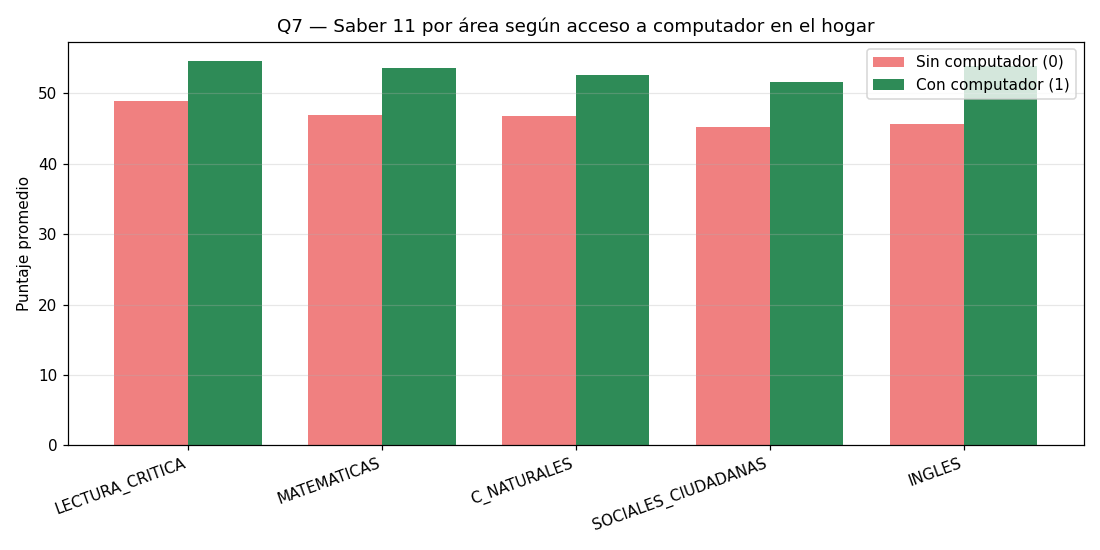
\includegraphics[width=0.85\textwidth]{figures/q7_computador_por_area.png}
\caption{Q7. Puntaje promedio por área evaluada según acceso a computador en el hogar.}
\end{figure}

\subsection{Q8. Municipios con alta conectividad pero bajos resultados académicos}
Se identificaron como anómalos los municipios que, en el año más reciente disponible (2022), cumplen simultáneamente dos condiciones: penetración de internet por encima del percentil 75 (umbral $\geq 0.624$) y puntaje global promedio por debajo del percentil 25 (umbral $\leq 223.93$). Solo 10 municipios cumplen ambas condiciones.

\begin{table}[H]
\centering
\caption{Municipios anómalos: alta conectividad y bajo puntaje (año 2022).}
\begin{tabular}{l l r r r r}
\toprule
\textbf{Cod} & \textbf{Departamento} & \textbf{N° est.} & \textbf{Puntaje} & \textbf{\% Internet} & \textbf{Idx. priv.} \\
\midrule
05736 & ANTIOQUIA  & 734 & 215.82 & 0.733 & 5.05 \\
19573 & CAUCA      & 953 & 213.10 & 0.719 & 2.46 \\
05579 & ANTIOQUIA  & 902 & 219.60 & 0.710 & 3.65 \\
05604 & ANTIOQUIA  & 742 & 209.15 & 0.701 & 4.63 \\
05585 & ANTIOQUIA  & 252 & 215.92 & 0.698 & 3.06 \\
73275 & TOLIMA     & 576 & 220.58 & 0.688 & 3.31 \\
13160 & BOLIVAR    & 170 & 222.49 & 0.671 & 4.47 \\
05847 & ANTIOQUIA  & 806 & 222.60 & 0.660 & 3.74 \\
41016 & HUILA      & 402 & 218.84 & 0.637 & 3.18 \\
27810 & CHOCO      & 132 & 203.77 & 0.636 & 4.73 \\
\bottomrule
\end{tabular}
\end{table}

Los municipios anómalos se concentran de manera notable en \textbf{Antioquia} (5 de los 10 casos), un departamento con alta capacidad institucional pero con focos territoriales específicos donde la inversión en conectividad no ha logrado traducirse en mejoras académicas. Los otros departamentos representados son Cauca, Tolima, Bolívar, Huila y Chocó, lo que cubre regiones con perfiles socioeconómicos diversos.

Al comparar los patrones promedio de los municipios anómalos frente al resto del país en el mismo año (2022), se observa que la conectividad promedio del grupo anómalo (68.5\%) está muy por encima del resto (50.0\%), pero su puntaje promedio (216.19) es considerablemente inferior al del resto (238.56). El índice de privación promedio es similar entre los dos grupos (3.83 vs 3.87), lo que indica que la brecha no se explica únicamente por pobreza, sino por factores adicionales que pueden incluir calidad educativa, deserción más alta (5.1\% frente a 4.1\% del resto) o factores cualitativos no capturados directamente por las fuentes utilizadas en este estudio.

Este hallazgo refuerza la conclusión transversal de Q3, Q4 y Q5: la conectividad por sí sola no garantiza buenos resultados académicos cuando no va acompañada de un ecosistema educativo y socioeconómico funcional. Estos municipios constituyen un grupo objetivo prioritario para análisis cualitativos posteriores que permitan identificar qué intervenciones complementarias son necesarias para que la inversión en infraestructura digital se traduzca en mejoras académicas reales.
